\documentclass[aspectratio=169]{beamer}

\usetheme{Madrid}
\usecolortheme{spruce}
\setbeamertemplate{navigation symbols}{}

\usepackage{amsmath, amssymb, mathtools}
\usepackage{tikz}
\usetikzlibrary{automata, positioning, arrows.meta}
\usepackage[dvipsnames]{xcolor}

\newtheorem{proposition}{Proposition}

\title{Introduction to Computation Theory}
\subtitle{Lecture Slides 1--2}
\author{Vinsong}
\institute{NTU AMFL}
\date{\today}

\AtBeginSection[]{
  \begin{frame}[plain]
    \centering
    \vfill
    {\Huge\textcolor{ForestGreen!70!black}{\insertsection}}
    \vfill
  \end{frame}
  \begin{frame}{Section Map}
    \tableofcontents[currentsection,hideothersubsections]
  \end{frame}
}

\begin{document}

\begin{frame}
  \titlepage
\end{frame}

\begin{frame}{Course Roadmap}
  \tableofcontents
\end{frame}

\section{Lecture 1: Basic Knowledge}

\subsection{Overview}

\begin{frame}{Lecture 1 Goals}
  \begin{itemize}
    \item Review foundational mathematical objects needed for automata theory.
    \item Establish proof vocabulary and common proof strategies.
    \item Introduce deterministic finite automata and regular operations.
  \end{itemize}
\end{frame}

\subsection{Mathematical Notions}

\begin{frame}{Set Basics}
  \begin{definition}[Set]
    A set collects distinct elements without regard to order or multiplicity.
  \end{definition}
  \begin{itemize}
    \item $\{1,2,3\} = \{3,2,1\}$ because order is ignored.
    \item $\{1,1,2,3\} = \{1,2,3\}$ because repetition does not change membership.
  \end{itemize}
\end{frame}

\begin{frame}{Sequences and Tuples}
  \begin{definition}[Sequence]
    An ordered list of objects where order and repetition matter.
  \end{definition}
  \begin{definition}[Tuple]
    A finite sequence; $(1,2,3)$ is a $3$-tuple.
  \end{definition}
  \begin{itemize}
    \item $(1,2,3) \neq (2,1,3)$ since order differs.
    \item $(1,2,2)$ and $(1,2,3)$ are distinct because repetition counts.
  \end{itemize}
\end{frame}

\begin{frame}{Sets vs.\ Sequences}
  \begin{itemize}
    \item \textbf{Order}: ignored in sets, preserved in sequences.
    \item \textbf{Multiplicity}: collapsed in sets, tracked in sequences.
    \item Example:
      \[
        \text{Sequence } (1,1,2,3) \neq (1,2,3), \quad
        \text{Set } \{1,1,2,3\} = \{1,2,3\}.
      \]
  \end{itemize}
\end{frame}

\begin{frame}{Cartesian Product}
  \begin{definition}[Cartesian Product]
    $A \times B = \{(a,b) \mid a \in A, b \in B\}$.
  \end{definition}
  \begin{example}
    For $A=\{1,2\}$ and $B=\{x,y\}$,
    \[
      A \times B = \{(1,x),(1,y),(2,x),(2,y)\}.
    \]
  \end{example}
\end{frame}

\subsection{Functions and Relations}

\begin{frame}{Function as a Machine}
  \begin{definition}[Function]
    Associates each input with exactly one output.
  \end{definition}
  \begin{itemize}
    \item Domain: permissible inputs.
    \item Codomain: possible outputs.
    \item Think of a machine with a single exit.
  \end{itemize}
\end{frame}

\begin{frame}{Equivalence Relation}
  \begin{definition}[Equivalence Relation]
    A relation $R$ is equivalent when
    \begin{itemize}
      \item Reflexive: $\forall x,\; xRx$.
      \item Symmetric: $\forall x,y,\; xRy \Rightarrow yRx$.
      \item Transitive: $\forall x,y,z,\; xRy \land yRz \Rightarrow xRz$.
    \end{itemize}
  \end{definition}
\end{frame}

\begin{frame}{Example: Modulo 7}
  \begin{example}
    $i \equiv_{7} j$ if $i-j$ is divisible by $7$.
  \end{example}
  \begin{itemize}
    \item Reflexive: $i-i = 0 \equiv 0 \pmod{7}$.
    \item Symmetric: $i-j = 7a \Rightarrow j-i = -7a$.
    \item Transitive: $i-j = 7a$ and $j-k = 7b \Rightarrow i-k = 7(a+b)$.
  \end{itemize}
\end{frame}

\subsection{Strings and Languages}

\begin{frame}{Alphabet and Strings}
  \begin{itemize}
    \item \textbf{Alphabet}: finite set of symbols, e.g., $\{0,1\}$.
    \item \textbf{String}: finite sequence of symbols, e.g., $01000$.
  \end{itemize}
\end{frame}

\begin{frame}{Languages}
  \begin{definition}[Language]
    A set of strings over an alphabet. For machine $A$, write $L(A)$.
  \end{definition}
  \begin{itemize}
    \item Languages can be finite or infinite.
    \item Example: all binary strings ending with $01$.
  \end{itemize}
\end{frame}

\subsection{Definitions, Theorems, Proofs}

\begin{frame}{Terminology}
  \begin{itemize}
    \item \textbf{Definition}: introduces a new concept.
    \item \textbf{Statement}: a sentence that is true or false.
    \item \textbf{Theorem}: a statement proven true.
    \item \textbf{Lemma}: a helping theorem.
    \item \textbf{Corollary}: follows quickly from another theorem.
  \end{itemize}
\end{frame}

\begin{frame}{Proof by Construction}
  \begin{proposition}
    The sum of degrees of every graph is even.
  \end{proposition}
  \begin{proof}[Idea]
    Each edge touches two vertices, so
    \[
      \sum_{v \in V} \deg(v) = 2|E|,
    \]
    which is even.
  \end{proof}
  \begin{note}
    Relies on the definition of how edges contribute to degree.
  \end{note}
\end{frame}

\begin{frame}{Proof by Contradiction}
  \begin{itemize}
    \item Assume the statement is false.
    \item Deduce a contradiction.
    \item Conclude the original statement must be true.
  \end{itemize}
\end{frame}

\begin{frame}{Proof by Induction}
  \begin{itemize}
    \item Basis: prove the statement for a simple starting case, e.g., $n=0$ or $n=1$.
    \item Inductive Step: assume truth for $n=k$ and prove for $n=k+1$.
  \end{itemize}
\end{frame}

\subsection{Deterministic Finite Automata}

\begin{frame}{Automata Vocabulary}
  \begin{itemize}
    \item \textbf{Automaton}: a single machine.
    \item \textbf{Automata}: plural form.
  \end{itemize}
\end{frame}

\begin{frame}{Definition of DFA}
  \begin{definition}
    A DFA is a 5-tuple $(Q,\Sigma,\delta,q_0,F)$ where
    \begin{itemize}
      \item $Q$: finite set of states,
      \item $\Sigma$: finite alphabet,
      \item $\delta: Q \times \Sigma \to Q$,
      \item $q_0 \in Q$: start state,
      \item $F \subseteq Q$: accept states.
    \end{itemize}
  \end{definition}
\end{frame}

\begin{frame}{Example DFA}
  \begin{center}
    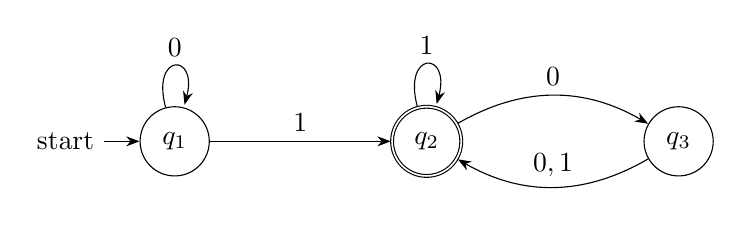
\begin{tikzpicture}[node distance=3.2cm, ->, >=Stealth, on grid, auto]
      \node[state, initial] (q1) {$q_1$};
      \node[state, accepting, right of=q1] (q2) {$q_2$};
      \node[state, right of=q2] (q3) {$q_3$};
      \path (q1) edge[loop above] node {$0$} (q1)
            (q1) edge node {$1$} (q2)
            (q2) edge[loop above] node {$1$} (q2)
            (q2) edge[bend left] node {$0$} (q3)
            (q3) edge[bend left] node[swap] {$0,1$} (q2);
    \end{tikzpicture}
  \end{center}
\end{frame}

\begin{frame}{Transition Function Table}
  \begin{center}
    \begin{tabular}{c|c c}
      & $0$ & $1$ \\ \hline
      $q_1$ & $q_1$ & $q_2$ \\
      $q_2$ & $q_3$ & $q_2$ \\
      $q_3$ & $q_2$ & $q_2$ \\
    \end{tabular}
  \end{center}
\end{frame}

\begin{frame}{Language of a Machine}
  \begin{definition}
    The language recognized by $M$ is $L(M) = A$. We say $A$ is accepted by $M$.
  \end{definition}
\end{frame}

\begin{frame}{Computation of a DFA}
  Let $M = (Q,\Sigma,\delta,q_0,F)$ and $w = w_1 \cdots w_n$.
  \begin{theorem}
    $M$ accepts $w$ if there exist states $r_0,\ldots,r_n$ such that
    \begin{enumerate}
      \item $r_0 = q_0$,
      \item $r_{i+1} = \delta(r_i, w_{i+1})$ for $0 \le i < n$,
      \item $r_n \in F$.
    \end{enumerate}
  \end{theorem}
\end{frame}

\begin{frame}{Regular Languages}
  \begin{definition}[Regular Language]
    A language is regular if it is recognized by some finite automaton.
  \end{definition}
\end{frame}

\begin{frame}{Regular Operations}
  Let $A$ and $B$ be languages.
  \begin{itemize}
    \item Union: $A \cup B = \{ w \mid w \in A \lor w \in B \}$.
    \item Concatenation: $A \circ B = \{ w_1w_2 \mid w_1 \in A,\ w_2 \in B \}$.
    \item Kleene Star: $A^* = \{ w_1 \cdots w_k \mid k \ge 0,\ w_i \in A \}$.
  \end{itemize}
\end{frame}

\begin{frame}{Kleene Star Detail}
  \[
    A^* = \{\epsilon\} \cup A \cup A^2 \cup A^3 \cup \cdots
  \]
  with
  \begin{itemize}
    \item $A^0 = \{\epsilon\}$,
    \item $A^n = \{ wv \mid w \in A^{n-1},\ v \in A \}$ for $n \ge 1$.
  \end{itemize}
\end{frame}

\begin{frame}{Closure Concepts}
  \begin{definition}[Closed Operation]
    An operation $R$ is closed on a set $A$ if $x,y \in A$ implies $xRy \in A$.
  \end{definition}
  \begin{theorem}
    Regular languages are closed under union, concatenation, and Kleene star.
  \end{theorem}
\end{frame}

\begin{frame}{Closure Under Union}
  Given
  \[
    M_1 =(Q_1, \Sigma, \delta_1, q_1, F_1), \quad
    M_2 =(Q_2, \Sigma, \delta_2, q_2, F_2),
  \]
  build product automaton
  \[
    M = (Q, \Sigma, \delta, q_0, F)
  \]
  with
  \begin{itemize}
    \item $Q = Q_1 \times Q_2$,
    \item $q_0 = (q_1,q_2)$,
    \item $\delta((r_1,r_2),a) = (\delta_1(r_1,a),\delta_2(r_2,a))$,
    \item $F = \{(r_1,r_2) \mid r_1 \in F_1 \text{ or } r_2 \in F_2\}$.
  \end{itemize}
  Then $L(M) = L(M_1) \cup L(M_2)$.
\end{frame}

\section{Lecture 2: Nondeterminism}

\subsection{Overview}

\begin{frame}{Lecture 2 Goals}
  \begin{itemize}
    \item Define nondeterministic finite automata (NFAs).
    \item Show equivalence between NFAs and DFAs.
    \item Construct NFAs for union, concatenation, and Kleene star.
  \end{itemize}
\end{frame}

\subsection{NFA Intuition}

\begin{frame}{Sample NFA}
  \begin{center}
    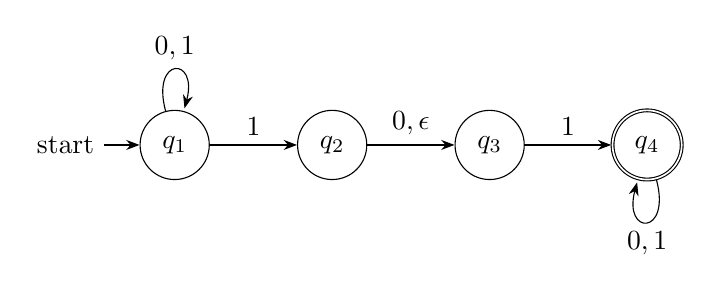
\begin{tikzpicture}[->, node distance=2cm, >=Stealth, on grid, auto]
      \node[state, initial] (q1) {$q_1$};
      \node[state] (q2) [right of=q1] {$q_2$};
      \node[state] (q3) [right of=q2] {$q_3$};
      \node[state, accepting] (q4) [right of=q3] {$q_4$};
      \path (q1) edge[loop above] node {$0,1$} (q1)
            (q1) edge node {$1$} (q2)
            (q2) edge node {$0,\epsilon$} (q3)
            (q3) edge node {$1$} (q4)
            (q4) edge[loop below] node {$0,1$} (q4);
    \end{tikzpicture}
  \end{center}
  \begin{itemize}
    \item Accepts strings with a $1$ in the third position from the end.
    \item $\delta(q_1,1)$ returns $q_1$ or $q_2$.
    \item $\epsilon$ between $q_2$ and $q_3$ consumes no input.
  \end{itemize}
\end{frame}

\begin{frame}{Determinizing the Example}
  \begin{center}
    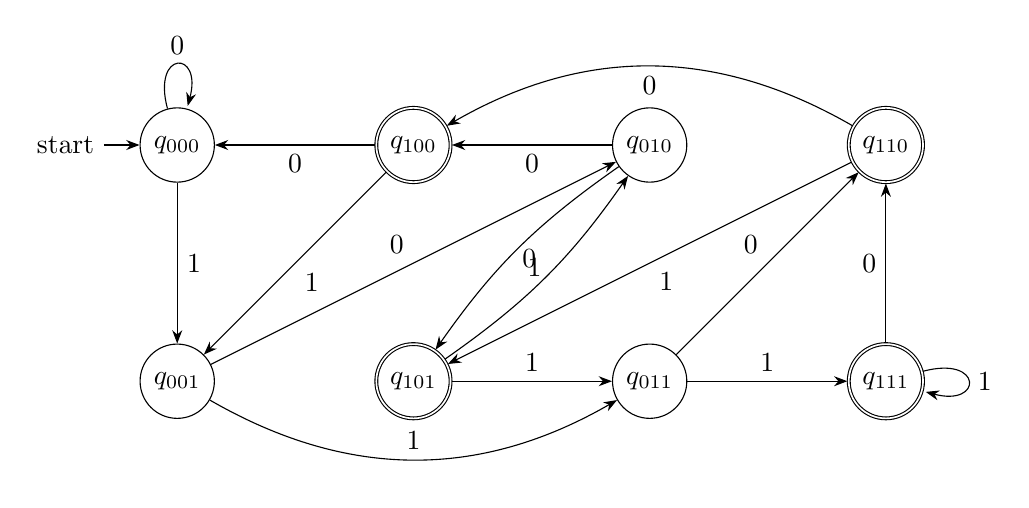
\begin{tikzpicture}[->, node distance=3cm, >=Stealth, on grid, auto]
      \node[state, initial] (s000) {$q_{000}$};
      \node[state, accepting, right of=s000] (s100) {$q_{100}$};
      \node[state, right of=s100] (s010) {$q_{010}$};
      \node[state, accepting, right of=s010] (s110) {$q_{110}$};
      \node[state, below of=s000] (s001) {$q_{001}$};
      \node[state, accepting, right of=s001] (s101) {$q_{101}$};
      \node[state, right of=s101] (s011) {$q_{011}$};
      \node[state, accepting, right of=s011] (s111) {$q_{111}$};
      \path (s000) edge[loop above] node {$0$} (s000)
            (s000) edge node {$1$} (s001)
            (s100) edge node {$0$} (s000)
            (s100) edge node {$1$} (s001)
            (s010) edge[bend right=10] node {$1$} (s101)
            (s010) edge node {$0$} (s100)
            (s110) edge[bend right] node {$0$} (s100)
            (s110) edge node {$1$} (s101)
            (s001) edge[bend right] node {$1$} (s011)
            (s001) edge node {$0$} (s010)
            (s101) edge[bend right=10] node {$0$} (s010)
            (s101) edge node {$1$} (s011)
            (s011) edge node {$1$} (s111)
            (s011) edge node {$0$} (s110)
            (s111) edge[loop right] node {$1$} (s111)
            (s111) edge node {$0$} (s110);
    \end{tikzpicture}
  \end{center}
  \begin{itemize}
    \item Subset construction encodes sets of NFA states as DFA states.
    \item May require up to $2^{|Q|}$ deterministic states.
  \end{itemize}
\end{frame}

\subsection{Formal Definitions}

\begin{frame}{Power Set Reminder}
  \begin{definition}[Power Set]
    $P(Q) = \{ X \mid X \subseteq Q \}$ contains all $2^{|Q|}$ subsets of $Q$.
  \end{definition}
\end{frame}

\begin{frame}{Definition of NFA}
  \begin{definition}[NFA]
    $M = (Q,\Sigma_{\epsilon},\delta,q_0,F)$ with
    \begin{itemize}
      \item $Q$: finite set of states,
      \item $\Sigma_{\epsilon} = \Sigma \cup \{\epsilon\}$,
      \item $\delta: Q \times \Sigma_{\epsilon} \to P(Q)$,
      \item $q_0 \in Q$,
      \item $F \subseteq Q$.
    \end{itemize}
  \end{definition}
\end{frame}

\begin{frame}{Acceptance in an NFA}
  Take $w = y_1 \cdots y_m$ with $y_i \in \Sigma_{\epsilon}$.
  \begin{theorem}
    $M$ accepts $w$ if there exist states $r_0,\ldots,r_m$ such that
    \begin{enumerate}
      \item $r_0 = q_0$,
      \item $r_{i+1} \in \delta(r_i, y_{i+1})$ for $0 \le i < m$,
      \item $r_m \in F$.
    \end{enumerate}
  \end{theorem}
  \begin{note}
    The sequence length $m$ may differ from the input length because $\epsilon$-moves consume no symbols.
  \end{note}
\end{frame}

\subsection{Equivalence of DFA and NFA}

\begin{frame}{DFA as NFA}
  \begin{itemize}
    \item A DFA is an NFA with no true nondeterminism.
    \item Add $\delta(q,\epsilon) = \emptyset$ to align alphabets: $\Sigma \subset \Sigma_{\epsilon}$.
  \end{itemize}
\end{frame}

\begin{frame}{Example NFA}
  \begin{center}
    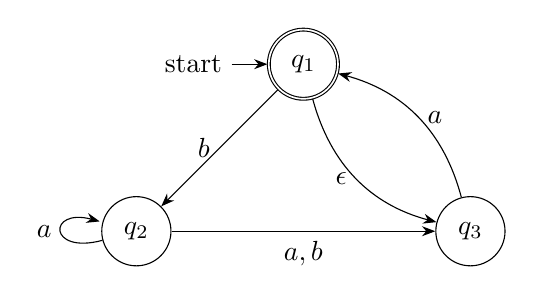
\begin{tikzpicture}[->, node distance=3cm, >=Stealth, on grid, auto]
      \node[state, initial, accepting] (q1) {$q_1$};
      \node[state, below left of=q1] (q2) {$q_2$};
      \node[state, below right of=q1] (q3) {$q_3$};
      \path (q1) edge node[left] {$b$} (q2)
            (q2) edge[loop left] node {$a$} (q2)
            (q1) edge[bend right] node[left] {$\epsilon$} (q3)
            (q2) edge node[below] {$a,b$} (q3)
            (q3) edge[bend right] node[right] {$a$} (q1);
    \end{tikzpicture}
  \end{center}
\end{frame}

\begin{frame}{Subset Construction Result}
  \begin{center}
    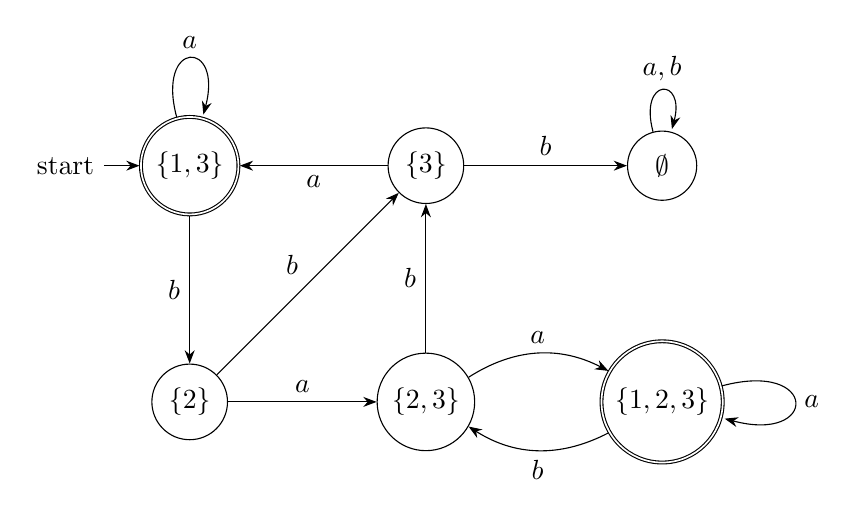
\begin{tikzpicture}[->, node distance=3cm, >=Stealth, on grid, auto]
      \node[state, initial, accepting, initial where=left] (s13) {$\{1,3\}$};
      \node[state, below of=s13] (s2) {$\{2\}$};
      \node[state, right of=s13] (s3) {$\{3\}$};
      \node[state, right of=s3] (sphi) {$\emptyset$};
      \node[state, right of=s2] (s23) {$\{2,3\}$};
      \node[state, accepting, right of=s23] (s123) {$\{1,2,3\}$};
      \path (sphi) edge[loop above] node {$a,b$} (sphi)
            (s2) edge node {$a$} (s23)
            (s2) edge node {$b$} (s3)
            (s3) edge node {$b$} (sphi)
            (s3) edge node {$a$} (s13)
            (s13) edge[loop above] node {$a$} (s13)
            (s13) edge node[left] {$b$} (s2)
            (s23) edge[bend left] node {$a$} (s123)
            (s23) edge node {$b$} (s3)
            (s123) edge[loop right] node {$a$} (s123)
            (s123) edge[bend left] node {$b$} (s23);
    \end{tikzpicture}
  \end{center}
\end{frame}

\begin{frame}{Refining the Converted DFA}
  \begin{itemize}
    \item Remove unreachable subsets.
    \item Include all $\epsilon$-reachable states in the start subset:
      \[
        \{q_1\} \ \text{(wrong)} \quad \to \quad \{q_1,q_3\} \ \text{(correct)}.
      \]
  \end{itemize}
\end{frame}

\begin{frame}{Epsilon-Closure}
  \begin{definition}
    $E(\{q_0\}) = \{q_0\} \cup \{\text{states reachable by }\epsilon \text{ from } q_0\}$.
  \end{definition}
\end{frame}

\begin{frame}{Subset Construction Theorem}
  Given NFA $M = (Q,\Sigma,\delta,q_0,F)$, define DFA $M' = (Q',\Sigma,\delta',q_0',F')$ with
  \begin{itemize}
    \item $Q' = P(Q)$,
    \item $q_0' = E(\{q_0\})$,
    \item $F' = \{ R \mid R \cap F \neq \emptyset \}$,
    \item $\delta'(R,a) = \displaystyle\bigcup_{r \in R} E(\delta(r,a))$.
  \end{itemize}
\end{frame}

\subsection{Closure via NFAs}

\begin{frame}{NFA Building Blocks}
  Take $N_1 =(Q_1,\Sigma,\delta_1,q_1,F_1)$ and $N_2 =(Q_2,\Sigma,\delta_2,q_2,F_2)$ with $\epsilon \notin \Sigma$.
  \begin{center}
    \begin{tabular}{c c c}
      $N_1$ && $N_2$ \\
      \begin{tikzpicture}[node distance=1.6cm, every node/.style={scale=0.55}]
        \node[state, initial] (1) {$q_1$};
        \node[state, above right=of 1, yshift=-0.8cm] (2) {};
        \node[state, below right=of 1, yshift=0.8cm] (3) {};
        \node[state, right=of 1, xshift=0.7cm] (6) {};
        \node[state, accepting, above right=of 6, yshift=-0.6cm] (4) {};
        \node[state, accepting, below right=of 6, yshift=0.6cm] (5) {};
      \end{tikzpicture}
      &&
      \begin{tikzpicture}[node distance=1.6cm, every node/.style={scale=0.55}]
        \node[state, initial] (01) {$q_2$};
        \node[state, above right=of 01, yshift=-0.8cm] (02) {};
        \node[state, below right=of 01, yshift=0.7cm] (03) {};
        \node[state, right=of 01, xshift=0.5cm] (06) {};
        \node[state, accepting, above right=of 06, yshift=-0.6cm] (04) {};
        \node[state, accepting, below right=of 06, yshift=0.6cm] (05) {};
        \node[state, accepting, right=of 06, xshift=0.8cm] (07) {};
      \end{tikzpicture}
    \end{tabular}
  \end{center}
\end{frame}

\begin{frame}{Union Construction (Diagram)}
  \begin{center}
    \begin{tikzpicture}[node distance=1.8cm, every node/.style={scale=0.55}, ->, >=Stealth, on grid, auto]
      \node[state, initial] (0) {$q_0$};
      \node[state, above right=of 0] (1) {$q_1$};
      \node[state, below right=of 0] (01) {$q_2$};
      \node[state, right=of 1, xshift=0.7cm] (6) {};
      \node[state, accepting, above right=of 6, yshift=-0.6cm] (4) {};
      \node[state, accepting, below right=of 6, yshift=0.6cm] (5) {};
      \node[state, right=of 01, xshift=0.7cm] (06) {};
      \node[state, accepting, above right=of 06, yshift=-0.6cm] (04) {};
      \node[state, accepting, below right=of 06, yshift=0.6cm] (05) {};
      \path (0) edge node {$\epsilon$} (1);
      \path (0) edge node[swap] {$\epsilon$} (01);
    \end{tikzpicture}
  \end{center}
\end{frame}

\begin{frame}{Union Construction (Formal)}
  \begin{proposition}[Union]
    \[
      N_1 \cup N_2 = (Q,\Sigma,\delta,q_0,F)
    \]
    where
    \begin{itemize}
      \item $Q = Q_1 \cup Q_2 \cup \{q_0\}$,
      \item $\delta(q,a) =
        \begin{cases}
          \delta_1(q,a) & q \in Q_1, \\
          \delta_2(q,a) & q \in Q_2, \\
          \{q_1,q_2\} & q = q_0,\ a = \epsilon, \\
          \emptyset & q = q_0,\ a \neq \epsilon,
        \end{cases}$
      \item $F = F_1 \cup F_2$.
    \end{itemize}
  \end{proposition}
\end{frame}

\begin{frame}{Concatenation Construction (Diagram)}
  \begin{center}
    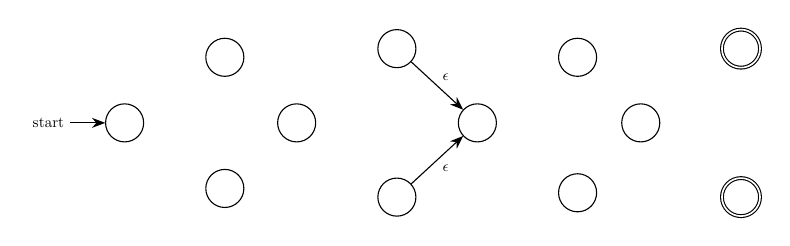
\begin{tikzpicture}[node distance=1.8cm, every node/.style={scale=0.55}, ->, >=Stealth, on grid, auto]
      \node[state, initial] (1) {};
      \node[state, above right=of 1, yshift=-0.8cm] (2) {};
      \node[state, below right=of 1, yshift=0.8cm] (3) {};
      \node[state, right=of 1, xshift=0.7cm] (6) {};
      \node[state, above right=of 6, yshift=-0.6cm] (4) {};
      \node[state, below right=of 6, yshift=0.6cm] (5) {};
      \node[state, right=of 6, xshift=0.9cm] (01) {};
      \node[state, above right=of 01, yshift=-0.8cm] (02) {};
      \node[state, below right=of 01, yshift=0.7cm] (03) {};
      \node[state, right=of 01, xshift=0.5cm] (06) {};
      \node[state, accepting, above right=of 06, yshift=-0.6cm] (04) {};
      \node[state, accepting, below right=of 06, yshift=0.6cm] (05) {};
      \path (4) edge node {$\epsilon$} (01);
      \path (5) edge node[swap] {$\epsilon$} (01);
    \end{tikzpicture}
  \end{center}
\end{frame}

\begin{frame}{Concatenation Construction (Formal)}
  \begin{proposition}[Concatenation]
    \[
      N_1 \circ N_2 = (Q,\Sigma,\delta,q_0,F)
    \]
    where
    \begin{itemize}
      \item $Q = Q_1 \cup Q_2$,
      \item $\delta(q,a) =
        \begin{cases}
          \delta_1(q,a) & q \in Q_1 \setminus F_1, \\
          \delta_2(q,a) & q \in Q_2, \\
          \delta_1(q,\epsilon) \cup \{q_2\} & q \in F_1,\ a = \epsilon, \\
          \delta_1(q,\epsilon) & q \in F_1,\ a \neq \epsilon,
        \end{cases}$
      \item $q_0 = q_1$,
      \item $F = F_2$.
    \end{itemize}
  \end{proposition}
\end{frame}

\begin{frame}{Kleene Star Construction (Diagram)}
  \begin{center}
    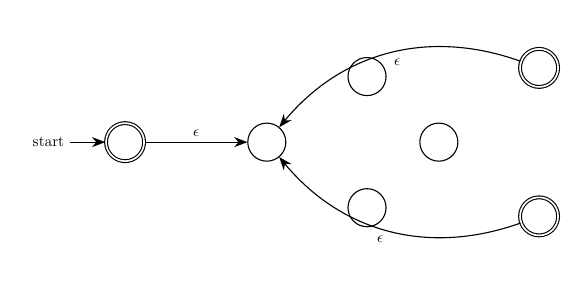
\begin{tikzpicture}[node distance=1.8cm, every node/.style={scale=0.55}, ->, >=Stealth, on grid, auto]
      \node[state, initial, accepting] (0) {};
      \node[state, right=of 0] (1) {};
      \node[state, above right=of 1, yshift=-0.8cm] (2) {};
      \node[state, below right=of 1, yshift=0.8cm] (3) {};
      \node[state, right=of 1, xshift=0.7cm] (6) {};
      \node[state, accepting, above right=of 6, yshift=-0.6cm] (4) {};
      \node[state, accepting, below right=of 6, yshift=0.6cm] (5) {};
      \path (4) edge[bend right=35] node {$\epsilon$} (1);
      \path (5) edge[bend left=35] node {$\epsilon$} (1);
      \path (0) edge node {$\epsilon$} (1);
    \end{tikzpicture}
  \end{center}
\end{frame}

\begin{frame}{Kleene Star Construction (Formal)}
  \begin{proposition}[Kleene Star]
    \[
      N_1^* = (Q,\Sigma,\delta,q_0,F)
    \]
    where
    \begin{itemize}
      \item $Q = Q_1 \cup \{q_0\}$,
      \item $\delta(q,a) =
        \begin{cases}
          \delta_1(q,a) & q \in Q_1 \setminus F_1, \\
          \delta_1(q,a) \cup \{q_1\} & q \in F_1,\ a = \epsilon, \\
          \delta_1(q,\epsilon) & q \in F_1,\ a \neq \epsilon, \\
          \{q_1\} & q = q_0,\ a = \epsilon, \\
          \emptyset & q = q_0,\ a \neq \epsilon,
        \end{cases}$
      \item $F = F_1 \cup \{q_0\}$.
    \end{itemize}
  \end{proposition}
\end{frame}

\begin{frame}{Additional Closure Notes}
  Regular languages are also closed under
  \begin{itemize}
    \item \textbf{Intersection}: accept when both components of the product automaton accept.
    \item \textbf{Set Difference}: accept when in $F_1$ but not $F_2$.
    \item \textbf{Complement}: $A_1^c = \Sigma^* - A_1$; difference preserves regularity.
  \end{itemize}
\end{frame}

\section{Wrap Up}

\begin{frame}{Key Takeaways}
  \begin{itemize}
    \item Lecture 1 established sets, sequences, proof methods, and deterministic automata.
    \item Lecture 2 introduced nondeterminism, subset construction, and NFA-based closures.
    \item Regular languages remain closed under core operations in both DFA and NFA settings.
  \end{itemize}
\end{frame}

\end{document}
